\newcommand{\uL}{\mathbf{L_0}}
\newcommand{\bL}{\mathbf{\bar{L}_0}}
\begin{columns}[T]
\begin{column}{.4\textwidth}
\begin{block}{Conformal Weights}
\vskip0.5cm
%\begin{tabular*}{\columnwidth}{@{\extracolsep{\stretch{1}}}*{2}{c}@{}}
%\begin{tabularx}{\columnwidth}{|X|X|}
%\toprule
\begin{align*}
	\mathbf{P} &=\frac{2\pi}{L}(\uL-\bL)  \\
	& = \frac{2\pi}{L}(em + n - \bar{n}) \\
	\widetilde{\mathbf{P}}&= em + n - \bar{n}\\ 
	\mathbf{H} &= \frac{2\pi}{L}(\uL+\bL)  \\
	&= \frac{2\pi}{L}(\frac{\kappa e^2}{2} + \frac{m^2}{2 \kappa} + \frac{n + \bar{n}}{2}) \\
	\widetilde{\mathbf{H}} &= \frac{L}{2 \pi \kappa}\mathbf{H} \\
&	= e^2 + \frac{m^2}{4 \kappa^2} + \frac{1}{\kappa}(n + \bar{n})
%\bottomrule
%\end{tabular*}
%\end{tabularx}
\end{align*}
\end{block}

%\begin{tabular}{lr}
%
%	$\mathbf{P} =\frac{2\pi}{L}(\uL-\bL)$ & 
%	$\frac{2\pi}{L}(em + n - \bar{n})$ \\
%	&
%	\\
%	$\widetilde{\mathbf{P}}$  &
%	$(em + n - \bar{n})$\\
%	& 
%	\\
%	$\mathbf{H} = \frac{2\pi}{L}(\uL+\bL)$ &
%	 $\frac{2\pi}{L}(\frac{\kappa e^2}{2} + \frac{m^2}{2 \kappa} + \frac{n + \bar{n}}{2})$ \\
%	&
%	 \\
%	$\widetilde{\mathbf{H}} = \frac{L}{2 \pi \kappa}\mathbf{H}$ &
%	 $e^2 + \frac{m^2}{4 \kappa^2} + \frac{1}{\kappa}(n + \bar{n})$       
%	\end{tabular}
	%\label{Table:EV}
	%\caption{Eigenvalues of states $\ket{e, m}_{n, \bar{n}}$.} 
	%\end{table}

\end{column}
\begin{column}{.6\textwidth}

\begin{block}{Conformal Charge}
\vskip4cm
	\begin{figure}[hbctp]
	\centering
	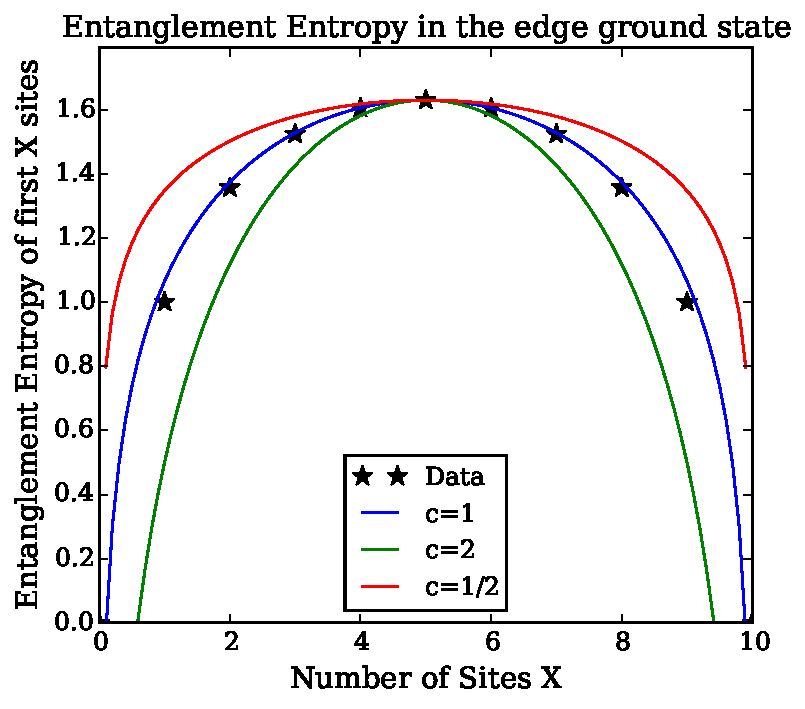
\includegraphics{{interpolatedboson/a0/plots/edge_gs_EE.pdf}}
	%\caption{Entanglement entropy within the entanglement ground state of the soft-core boson state on $10$ sites. For comparison, the Cardy-Calabrese formula $S(x) = c/3 \log \sin( \pi x/L) + const.$ is shown with $c=\frac{1}{2}, 1,$ and $2$, with the $const.$ fixed by matching the maximum of the entanglement entropy data. $c=1$ is a good fit.}
	%\label{fig:hc-edge-gs-ee}
	\end{figure}
%	\begin{figure}
%	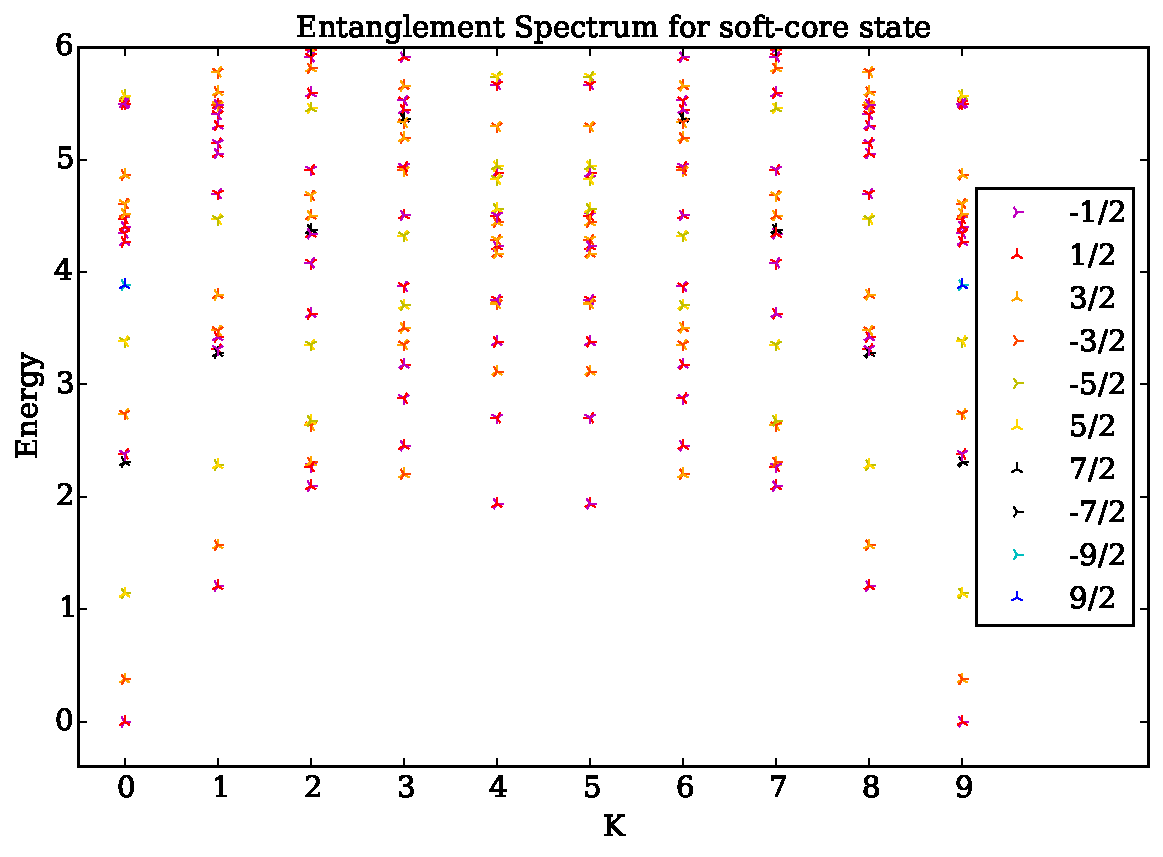
\includegraphics[width=\textwidth]{{interpolatedboson/new_plots/L_9_all_mom_10.pdf}}
%	\end{figure}
\end{block}
\end{column}
\end{columns}
